\section{Stage 3: Manage your dependencies with Bower}

\begin{frame}[fragile]
  \begin{center}
    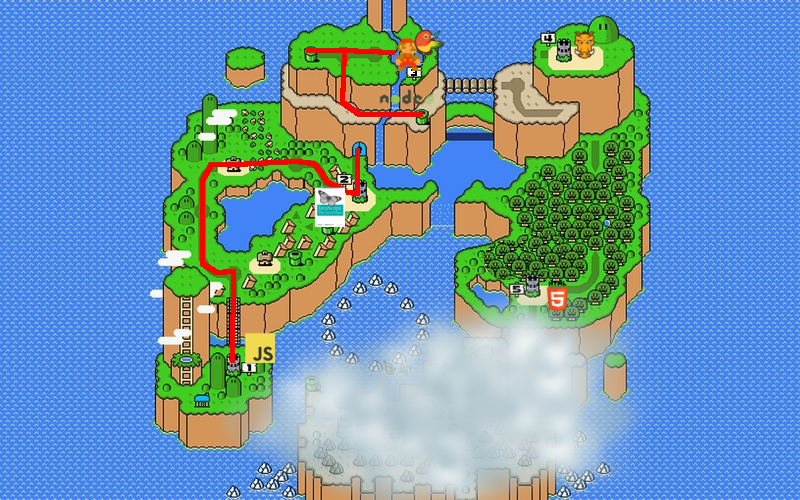
\includegraphics[width=300px]{images/map_stage_3.png}
  \end{center}
\end{frame}

\begin{frame}[fragile]
  \frametitle{What is Bower?}
  \begin{block}{Website definition}
    Bower is a package manager for the web. It offers a generic, unopinionated solution to the problem of front-end package management, while exposing the package dependency model via an API that can be consumed by a more opinionated build stack. 
  \end{block}

  \begin{center}
    
\includegraphics[width=100px]{images/bower-logo.png}
  \end{center}
\end{frame}

\begin{frame}[fragile]
  \frametitle{Installation}

  \begin{block}{Using npm}
  {\scriptsize
    \begin{verbatim}
    $ npm install -g bower
    \end{verbatim}
  }
  \end{block}

  \pause

  \begin{block}{Verify installation}
  {\scriptsize
    \begin{verbatim}
    $ bower -v
    1.2.7
    \end{verbatim}
  }
  \end{block}
\end{frame}

\begin{frame}[fragile]
  \frametitle{Commands}

  \begin{block}{\texttt{bower init}}
    Creates a bower.json file for including our application dependencies. Also, it's mandatory in order to register our application as a bower package or used on our internal projects through bower.
    {\tiny
    \begin{verbatim}
    $ bower init
    // Press ENTER for default answers
    $ cat bower.json
    {
      ``name'': ``js-workshop-code'',
      ``version'': ``0.0.0'',
      ``homepage'': ``https://github.com/ultrayoshi/js-workshop-code'',
      ``authors'': [
        ``ultrayoshi <david@imesmes.com>''
      ],
      ``license'': ``MIT'',
      ``ignore'': [
        ``**/.*'',
        ``node_modules'',
        ``bower_components'',
        ``test'',
        ``tests''
      ]
    }
    \end{verbatim}
    }
  \end{block}
\end{frame}

\begin{frame}[fragile]
  \frametitle{Commands}

  \begin{block}{\texttt{bower search}}
    Find all packages or a specific package
    {\tiny
    \begin{verbatim}
    $ bower search jquery
    Search results:
        jquery git://github.com/components/jquery.git
        jquery-ui git://github.com/components/jqueryui
        jquery.cookie git://github.com/carhartl/jquery-cookie.git
        jquery-placeholder git://github.com/mathiasbynens/jquery-placeholder.git
        jquery-file-upload git://github.com/blueimp/jQuery-File-Upload.git
        jasmine-jquery git://github.com/velesin/jasmine-jquery
        jquery.ui git://github.com/jquery/jquery-ui.git
        jquery.scrollTo git://github.com/flesler/jquery.scrollTo.git
        jquery-migrate git://github.com/appleboy/jquery-migrate.git
        jquery-waypoints git://github.com/imakewebthings/jquery-waypoints.git
        ...
    \end{verbatim}
    }
  \end{block}

  \pause

  \begin{block}{\texttt{bower home <package>}}
    Opens a package homepage into your favorite browser
    {\tiny
    \begin{verbatim}
    $ bower home jquery
    \end{verbatim}
    }
  \end{block}
\end{frame}

\begin{frame}[fragile]
  \frametitle{Commands}

  \begin{block}{\texttt{bower install [package]}}
    Install a package locally
    {\tiny
    \begin{verbatim}
    $ bower install jquery --save-dev
    bower jquery#*                  cached git://github.com/components/jquery.git#2.0.3
    bower jquery#*                validate 2.0.3 against git://github.com/components/jquery.git#*
    bower jquery#~2.0.3            install jquery#2.0.3

    jquery#2.0.3 bower_components/jquery
    \end{verbatim}
    }
    \texttt{--save-dev} option add the package as a dependency of your application.
    Leave package name blank in order to install all your dependencies.
  \end{block}

  \pause

  \begin{block}{\texttt{bower list}}
    List local packages

    {\tiny
    \begin{verbatim}
    $ bower list
    bower check-new     Checking for new versions of the project dependencies..
    js-workshop-code#0.0.0 /home/david/code/js-workshop-code
    └── jquery#2.0.3
    \end{verbatim}
    }
  \end{block}
\end{frame}
